\documentclass[11pt,a4paper]{article}

\usepackage[utf8]{inputenc}
\usepackage[T1]{fontenc}
\usepackage[english]{babel}
\usepackage[margin=2.3cm]{geometry}
\usepackage{amsmath}
\usepackage{amssymb}
\usepackage{booktabs}
\usepackage{graphicx}
\usepackage{hyperref}
\usepackage{caption}
\usepackage{enumitem}
\usepackage{float}
\usepackage{algorithm}
\usepackage{algpseudocode}
\usepackage{tikz}
\usetikzlibrary{arrows.meta,positioning,shapes.geometric,fit,calc}

\hypersetup{colorlinks=true, linkcolor=blue, urlcolor=blue, citecolor=blue}
\captionsetup{font=small}

\title{\textbf{Report --- High Performance Computing} \\[0.2cm]
\large Project \texttt{s4t-trust-hpc}: Distributed Verification of ECDSA Signatures}
\author{Andrea Di Marco}
\date{}

\begin{document}
\maketitle
\vspace{-0.4cm}

% =====================================================
\section{Introduction and Measurement Environments}

The compute-intensive workload in this project is the batch verification of ECDSA digital signatures on the NIST P-256 elliptic curve. In the \texttt{s4t-trust-hpc} platform, this operation is executed during device onboarding to determine whether an incoming IoT device is authentic before registration on an immutable ledger. 

This report evaluates data and task parallelism across two execution environments:
\begin{enumerate}[nosep]
    \item \textbf{Isolated benchmark (containerized):} An environment composed of ephemeral Docker containers (\texttt{bench-worker-1..32}) hosted on a single physical workstation. Each container runs a standalone C++ gRPC service exposing the signature verification routine. The containers share a dedicated Docker bridge network with no external gateway or authentication dependencies.
    \item \textbf{Production chain (Stack4Things/IoTronic):} A three-stage pipeline orchestrating three containerized boards registered in an IoTronic deployment. Requests traverse a Keystone-authenticated REST interface, dispatch via a WAMP/Crossbar messaging bus to the Lightning-Rod agent on each board, and invoke local C++ workers via gRPC.
\end{enumerate}

\subsection{Separation of Experimental Datasets}

The experimental evaluations in this report distinguish two separate measurement campaigns:
\begin{itemize}[nosep]
    \item \textbf{M13 Campaign (Controlled Multi-Core Benchmark):} The primary campaign designed to evaluate the PCAM stages and architectural performance. All experiments (E0--E10) process a fixed batch of $N = 20{,}000$ signatures, repeated for 10 interleaved iterations per configuration under a constant CPU frequency governor (\texttt{performance}). Workload metrics use the verified baseline $T_1 = 1.0636$\,s (median of E0b).
    \item \textbf{M11.5 Campaign (Extended Scale Grid):} A secondary exploratory grid extending up to 32 worker containers with batches of 1,000 and 5,000 signatures (3 repetitions per point). In M11.5, containers were launched without hardware pinning, and RPC latency included unvectorized synthetic payload generation.
\end{itemize}
These two datasets are kept strictly separate and are not directly merged in cross-model comparisons.

\subsection{Hardware Environment}

All benchmarks run on an Intel Core i7-12700H host with 32\,GiB of DDR5 RAM running Linux kernel 6.8. The processor contains 14 physical cores organized into two microarchitectural clusters:
\begin{itemize}[nosep]
    \item 6 Performance cores (P-cores, Golden Cove), supporting 2 hardware threads each via Simultaneous Multi-Threading (SMT), mapped to logical CPUs 0--11.
    \item 8 Efficiency cores (E-cores, Gracemont), single-threaded, mapped to logical CPUs 12--19.
\end{itemize}
The machine exposes 20 logical execution units in total. Configurations utilizing more than 20 threads or processes enter oversubscription.

% =====================================================
\section{Problem and Sequential Algorithm}

The workload consists of verifying $N$ cryptographic signatures on the NIST P-256 elliptic curve. The input is a batch of $N$ independent records; each record contains a public key $Q$, a message $m$, and a signature $(r, s)$. The output is the count of records with valid signatures. The batch has no internal ordering, and individual verification tasks do not depend on one another.

\subsection{Verification of a Single Signature}

Let $G$ denote the base point of the NIST P-256 curve, $n$ its prime order, and $H$ the SHA-256 cryptographic hash function. Verifying one record proceeds according to Algorithm~\ref{alg:ecdsa_verify}.

\begin{algorithm}[H]
\caption{Sequential verification of one ECDSA signature}
\label{alg:ecdsa_verify}
\begin{algorithmic}[1]
\Require Public key $Q$, message $m$, signature $(r,s)$
\Ensure \textsc{valid} or \textsc{invalid}
\If{$r \notin [1, n-1]$ \textbf{or} $s \notin [1, n-1]$}
    \State \Return \textsc{invalid}
\EndIf
\State $e \gets H(m)$ \Comment{SHA-256 digest interpreted as integer}
\State $w \gets s^{-1} \bmod n$ \Comment{Modular inverse}
\State $u_1 \gets e \cdot w \bmod n,\quad u_2 \gets r \cdot w \bmod n$
\State $R \gets u_1 G + u_2 Q$ \Comment{Two scalar multiplications on curve}
\If{$R$ is the point at infinity}
    \State \Return \textsc{invalid}
\EndIf
\State \Return \textsc{valid} \textbf{if} $x_R \bmod n = r$ \textbf{else} \textsc{invalid}
\end{algorithmic}
\end{algorithm}

In the implementation, this operation is executed via OpenSSL's high-level EVP interface using the call pair \texttt{EVP\_DigestVerifyInit} (configured with SHA-256 and the EC key) and \texttt{EVP\_DigestVerify}, rather than an obsolete direct call to \texttt{ECDSA\_verify}. The two scalar multiplications in step 5 represent the dominant computational load. Figure~\ref{fig:verify_flow} outlines the logic following the preliminary range check.

\begin{figure}[H]
\centering
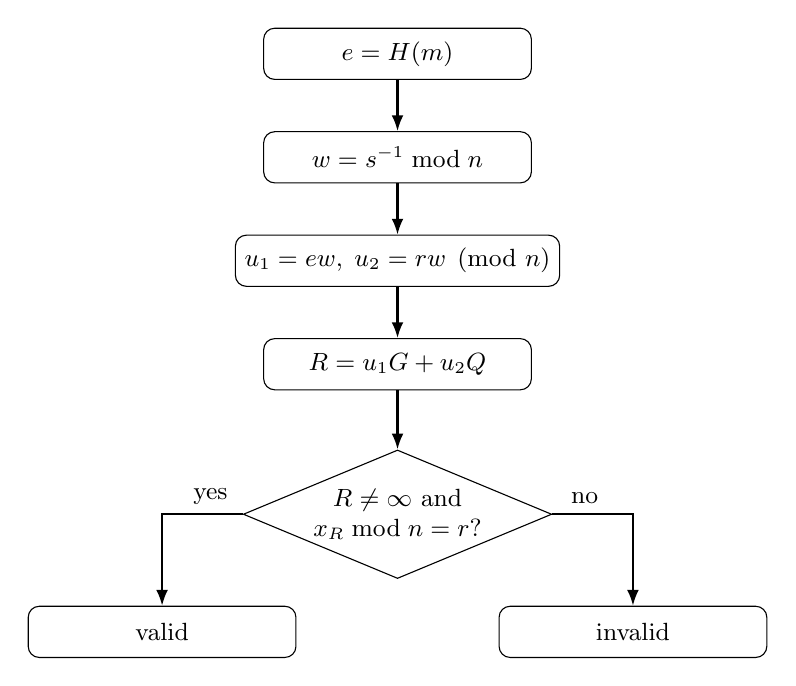
\begin{tikzpicture}[node distance=0.65cm, every node/.style={font=\small},
  box/.style={draw,rounded corners,minimum width=3.4cm,minimum height=0.65cm,align=center},
  dec/.style={draw,diamond,aspect=2.4,inner sep=1pt,align=center},
  arr/.style={-{Latex[length=2mm]},thick}]
\node[box] (a) {$e = H(m)$};
\node[box,below=of a] (b) {$w = s^{-1} \bmod n$};
\node[box,below=of b] (c) {$u_1 = e w,\; u_2 = r w \pmod n$};
\node[box,below=of c] (d) {$R = u_1 G + u_2 Q$};
\node[dec,below=0.75cm of d] (e) {$R \ne \infty$ and\\$x_R \bmod n = r$?};
\node[box,below left=0.75cm and 0.3cm of e] (v) {valid};
\node[box,below right=0.75cm and 0.3cm of e] (i) {invalid};
\draw[arr] (a)--(b); \draw[arr] (b)--(c); \draw[arr] (c)--(d); \draw[arr] (d)--(e);
\draw[arr] (e)-|node[above,pos=0.2]{yes}(v);
\draw[arr] (e)-|node[above,pos=0.2]{no}(i);
\end{tikzpicture}
\caption{Control flow of a single ECDSA verification after range checking.}
\label{fig:verify_flow}
\end{figure}

\subsection{Per-Verification Cost and Sequential Baseline}

To assess variability at the finest granularity, isolated execution times were measured across $20{,}000$ individual signature verifications (\texttt{per\_verify\_summary.csv}). The timer invocation overhead was measured at 12.8\,ns. 
The verification latency exhibits:
\begin{itemize}[nosep]
    \item Mean cost: $57.42\,\mu$s ($\text{standard deviation} = 7.27\,\mu$s)
    \item Coefficient of variation: $CV = 12.66\%$
    \item Median (p50): $55.71\,\mu$s, 90th percentile (p90): $59.73\,\mu$s, 99th percentile (p99): $87.44\,\mu$s
    \item Minimum: $50.79\,\mu$s, Maximum: $269.32\,\mu$s
\end{itemize}
Because $CV \approx 12.7\%$, individual tasks have nearly uniform computational duration.

Algorithm~\ref{alg:batch_verify} presents the reference sequential baseline. Its execution time over $N = 20{,}000$ signatures on a single P-core thread, compiled with \texttt{-O2}, defines the baseline $T_1 = 1.0636$\,s (median of 10 runs of E0b, with an interquartile range of 0.0031\,s, yielding $18{,}804.8$\,signatures/s). $T_1$ serves as the denominator for all speedup and efficiency values in the M13 campaign.

\begin{algorithm}[H]
\caption{Sequential batch verification (reference baseline, time $T_1$)}
\label{alg:batch_verify}
\begin{algorithmic}[1]
\Require Batch of $N$ records
\State $\textit{valid} \gets 0$
\For{$i = 0,\dots,N-1$}
  \State Allocate verification context (\texttt{EVP\_MD\_CTX})
  \If{\textsc{Verify}$(\text{record}_i)$ is valid}
    \State $\textit{valid} \gets \textit{valid} + 1$
  \EndIf
  \State Free verification context
\EndFor
\State Assert $\textit{valid} = N$ \Comment{Synthetic records are valid by construction}
\State \Return $\textit{valid}$
\end{algorithmic}
\end{algorithm}

\subsection{Profiling of the Sequential Code}\label{sec:profile}

The sequential algorithm was profiled using Valgrind Callgrind with OpenSSL debug symbols. Because Callgrind instruments machine instructions rather than sampling wall-clock time, results reflect the percentage of executed CPU instructions. Table~\ref{tab:callgrind_profile} and Figure~\ref{fig:profile_breakdown} summarize the instruction distribution for a batch of 500 signatures.

\begin{table}[H]
\centering\small
\begin{tabular}{lr}
\toprule
\textbf{Function / Region} & \textbf{\% Executed Instructions} \\
\midrule
\texttt{\_\_ecp\_nistz256\_mul\_montq} & 32.71\% \\
\texttt{\_\_ecp\_nistz256\_sqr\_montq} & 19.97\% \\
Other elliptic curve primitives & 14.48\% \\
\texttt{point\_double} + AVX2 & 7.71\% \\
BIGNUM operations (\texttt{BN\_uadd}, shift, div) & 7.10\% \\
\texttt{ord\_sqr\_mont} & 5.91\% \\
\midrule
Total Elliptic Curve and BIGNUM & \textbf{87.88\%} \\
Other cryptographic routines & 6.26\% \\
Memory management (\texttt{malloc}/\texttt{free}) & 3.20\% \\
Application logic & 1.80\% \\
\bottomrule
\end{tabular}
\caption{Flat instruction profile from Valgrind/Callgrind for sequential baseline (batch=500).}
\label{tab:callgrind_profile}
\end{table}

\begin{figure}[H]
\centering
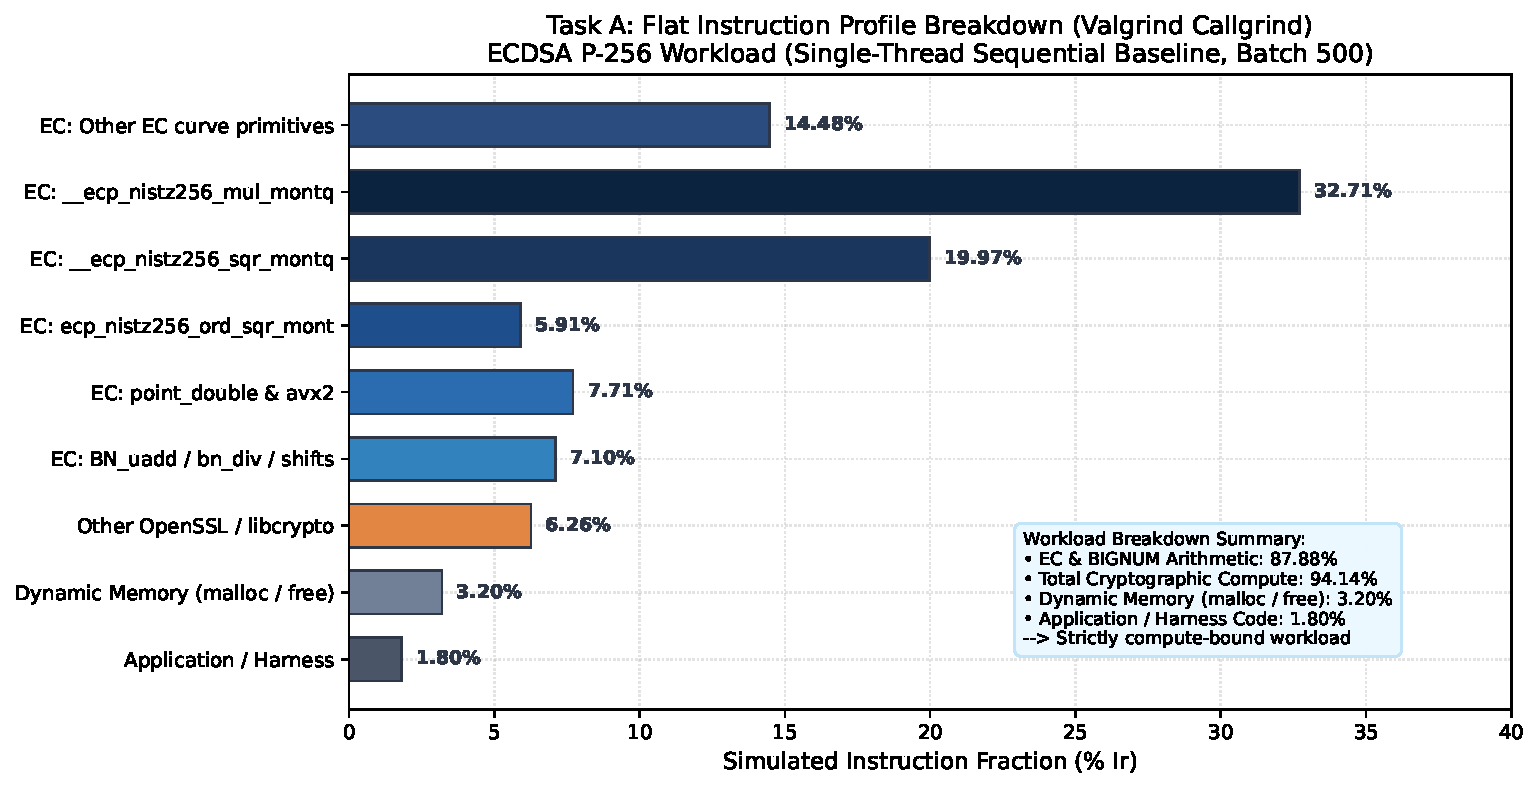
\includegraphics[width=0.82\textwidth]{figures/profile_breakdown.pdf}
\caption{Instruction breakdown from Callgrind profiling.}
\label{fig:profile_breakdown}
\end{figure}

Montgomery modular multiplication and squaring constitute 52.68\% of all executed instructions. In total, 87.88\% of instructions reside in elliptic-curve point arithmetic and multiprecision integer operations. Application logic accounts for only 1.80\%. 
This confirms that the execution time is governed by integer modular arithmetic, with negligible floating-point operations.

% =====================================================
\section{Partitioning}\label{sec:partitioning}

This section decomposes the signature verification problem into fine-grained tasks. The decomposition describes the structure of the computation independently of processes, threads, or communication protocols.

\subsection{Tasks and Data}

The computation is decomposed into two task types:
\begin{itemize}[nosep]
  \item \textbf{Verification task} $V_i$, for $i = 0, \dots, N-1$. Input: record $i$ (public key $Q$, message $m$, signature $(r,s)$). Output: binary decision $b_i \in \{0, 1\}$. Each $V_i$ executes Algorithm~\ref{alg:ecdsa_verify}.
  \item \textbf{Reduction task} $\Sigma$. Input: the set of decisions $\{b_0, \dots, b_{N-1}\}$. Output: total valid signatures $\sum_{i=0}^{N-1} b_i$.
\end{itemize}
Because each $V_i$ applies the identical verification operation to a distinct data record, the strategy is a domain decomposition. In the M13 experiments, $N = 20{,}000$, which is orders of magnitude larger than the number of hardware processing elements ($p \le 20$).

\subsection{Task Dependency Graph}

Figure~\ref{fig:dep_graph} illustrates the task dependency graph.

\begin{figure}[H]
\centering
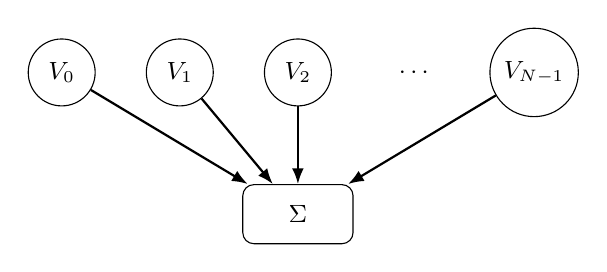
\begin{tikzpicture}[every node/.style={font=\small},
  t/.style={draw,circle,minimum size=0.85cm},
  s/.style={draw,rounded corners,minimum width=1.4cm,minimum height=0.75cm},
  arr/.style={-{Latex[length=2mm]},thick}]
\foreach \i/\l in {0/{V_0},1/{V_1},2/{V_2},4/{V_{N-1}}} {
  \node[t] (v\i) at (\i*1.5,0) {$\l$};
}
\node at (4.5,0) {$\cdots$};
\node[s] (r) at (3,-1.8) {$\Sigma$};
\foreach \i in {0,1,2,4} \draw[arr] (v\i)--(r);
\end{tikzpicture}
\caption{Task dependency graph for batch verification: $N$ concurrent tasks and one reduction. The critical path length is 2.}
\label{fig:dep_graph}
\end{figure}

The verification tasks are completely mutually independent. All dependency edges terminate at the reduction task $\Sigma$. Consequently, the maximum degree of concurrency is $N$, and the critical path consists of exactly one verification followed by the reduction.

\subsection{Task Interaction Graph}

Verification tasks do not exchange state during execution. The interaction graph contains no edges between any pair of verification tasks $(V_i, V_j)$. Interaction is confined to the fan-in to $\Sigma$, transferring one integer per group of tasks. Communication is therefore static, regular, and read-once.

\subsection{A Second Workload: The Three-Stage Pipeline}

The production platform incorporates a second workload characterized by functional pipelining: three sequential processing stages $S_1 \to S_2 \to S_3$, where the output of each stage feeds the next (Figure~\ref{fig:pipeline_graph}).

\begin{figure}[H]
\centering
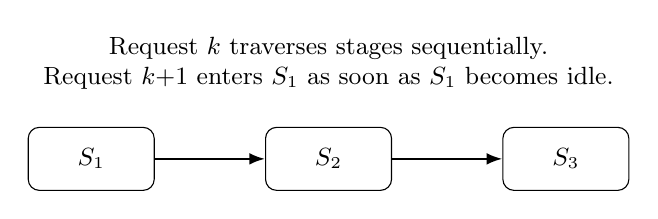
\begin{tikzpicture}[every node/.style={font=\small},
  s/.style={draw,rounded corners,minimum width=1.6cm,minimum height=0.8cm},
  arr/.style={-{Latex[length=2mm]},thick}]
\node[s] (a) {$S_1$}; \node[s,right=1.4cm of a] (b) {$S_2$}; \node[s,right=1.4cm of b] (c) {$S_3$};
\draw[arr] (a)--(b); \draw[arr] (b)--(c);
\node[above=0.35cm of b,align=center] {Request $k$ traverses stages sequentially.\\Request $k{+}1$ enters $S_1$ as soon as $S_1$ becomes idle.};
\end{tikzpicture}
\caption{Dependency and interaction graph for the three-stage functional pipeline.}
\label{fig:pipeline_graph}
\end{figure}

Unlike batch verification, the stages within a single request exhibit strict data dependencies and cannot run concurrently. Concurrency is achieved across multiple independent requests traversing the chain simultaneously.

% =====================================================
\section{Communication, Agglomeration, and Aggregation}

\subsection{Data Movement and Substrate Overhead}

In the batch workload, synthetic device records are generated deterministically from an integer seed directly on the computing node. No input dataset is transmitted across the network or memory bus; each worker receives only the seed, chunk size, and thread count. The return payload is limited to the partial valid count (an integer) and the elapsed execution time. Data movement is therefore restricted to a few bytes per chunk, independent of $N$.

Table~\ref{tab:comm_overhead} summarizes the measured communication substrates and their operational overheads.

\begin{table}[H]
\centering\small
\begin{tabular}{p{3.2cm}p{3.0cm}p{7.8cm}}
\toprule
\textbf{Substrate} & \textbf{Transport Mechanism} & \textbf{Measured Communication Overhead} \\
\midrule
MPI collective & Intra-node shared memory & Median \texttt{reduce\_s} measured at $0.038$\,ms (38\,$\mu$s on 8 bytes) \\
gRPC isolated & HTTP/2 over Docker bridge & Concurrent \texttt{Ping} latency: $1.1$--$1.3$\,ms \\
Production chain ($k=3$) & REST + WAMP + gRPC & $210$--$250$\,ms per stage ($\approx 690$\,ms steady-state transit). First invocation: $5.78$\,s (Keystone token and WAMP session handshake) \\
\bottomrule
\end{tabular}
\caption{Communication characteristics and measured overhead across execution substrates.}
\label{tab:comm_overhead}
\end{table}

\subsection{Agglomeration}

Assigning individual verification tasks ($V_i$) to separate messages or threads would incur scheduling and communication overheads far exceeding the $57.4\,\mu$s task duration. Tasks are therefore agglomerated into contiguous blocks. For a batch of $N$ records divided among $P$ processing groups, group $g \in \{0, \dots, P-1\}$ receives
\begin{equation}
n_g = \left\lfloor \frac{N}{P} \right\rfloor + \begin{cases} 1 & \text{if } g < N \bmod P \\ 0 & \text{otherwise} \end{cases}
\end{equation}
This partition guarantees that chunk sizes differ by at most one signature, maintaining load balance under uniform task durations. 

Agglomeration operates at two distinct tiers:
\begin{enumerate}[nosep]
  \item \textbf{Process/Container level:} The total batch $N$ is divided into $P$ chunks, one per MPI rank or gRPC container.
  \item \textbf{Thread level:} Within each rank or container, the chunk $n_g$ is sub-partitioned across OpenMP threads.
\end{enumerate}

\subsection{Aggregation}

Aggregation policies reflect the underlying concurrency model:
\begin{itemize}[nosep]
  \item \textbf{MPI Static:} Aggregation uses two collective reductions: \texttt{MPI\_SUM} over the valid signature counts, and \texttt{MPI\_MAX} over execution times (since the slowest rank defines the completion barrier).
  \item \textbf{MPI Dynamic (Master-Worker):} Rank 0 acts as a coordinator, receiving chunk completion messages and accumulating the valid count on demand. Workers report their maximum compute time via reduction at task completion.
  \item \textbf{gRPC Dispatch:} The client orchestrator invokes worker endpoints concurrently using Python's \texttt{asyncio.gather}. It accumulates the returned counts and asserts that the sum equals $N$, failing immediately upon missing data.
  \item \textbf{Production Pipeline:} State is chained sequentially between stages; each stage passes transformed data to its successor without collective reduction.
\end{itemize}

% =====================================================
\section*{6. Mapping}

In the MPI model, processes are launched with the \texttt{--bind-to none} option: Open MPI's default behaviour would bind each rank to a single physical core, which would prevent that rank's internal OpenMP threads from spreading across different cores and would force them to serialize, wasting part of the gain from the task+data hybrid discussed later. In the isolated benchmark, up to 32 \textit{worker} containers are mapped to as many dedicated host ports, in the range 51051--51082, so that each is individually reachable without addressing ambiguity. In the production pipeline, on the other hand, the mapping is static and fixed: the three boards registered on IoTronic correspond one to one to the three C++ workers connected on the \texttt{s4t-bridge} network, with no form of dynamic load balancing, a choice consistent with the fact that this environment is meant to measure the behaviour of the real chain as it is configured in production, not to explore alternative configurations.

% =====================================================
\section*{7. Performance evaluation}

The reference metrics are speedup $S_n = T_1/T_n$ and efficiency $E_n = S_n/n$, computed both with respect to the number of nodes and with respect to the effective parallelism $P_{eff} = \text{nodes} \times \text{threads}$, to separate the contribution of task parallelism from that of data parallelism when the two are combined.

\subsection*{7.1 Extended task parallelism: gRPC vs.\ MPI+OpenMP}

In the isolated benchmark, the experimental grid covers nodes in $\{1,2,4,8,16,32\}$, OpenMP threads per node in $\{1,2,4,8\}$, two batch sizes (1,000 and 5,000 signatures), three repetitions per configuration, with a correctness check on the total count for each of the 96 runs per substrate.

\begin{figure}[H]
\centering
\includegraphics[width=0.74\textwidth]{graphs/substrate_comparison_throughput_batch5000.pdf}
\caption{Maximum throughput per $P_{eff}$, gRPC vs.\ MPI+OpenMP (batch=5,000).}
\end{figure}

The two efficiency curves are comparable at equal effective parallelism, but the absolute throughput is not: MPI reaches an asymptote close to 164,000 signatures per second, against about 87,000 for gRPC dispatch. The difference is entirely explained by the communication cost of the substrate discussed in the previous section: MPI communicates through shared memory within the same host, gRPC pays the real cost of HTTP/2 framing and of traversing the network stack, even when the containers are on the same machine. It is the trade-off between tight and loose coupling: same algorithmic efficiency, different communication substrates, different price.

\subsection*{7.2 Amdahl's law}

The serial fraction $f_s = 2/S_2 - 1$ had been estimated in a previous calibration campaign at 2.51\%, from just two measurements at low parallelism. It was not recalculated in this campaign: the equivalent configuration on the new grid, two nodes with a 5,000-signature batch over three repetitions, shows a standard deviation of 21\% on the mean, too noisy a sample to support a reliable two-point estimate. It was therefore decided to reuse the value already validated.

\begin{table}[H]
\centering\small
\begin{tabular}{crrr}
\toprule
$P$ & Predicted & Measured & Gap \\
\midrule
4 (calibration) & 3.72$\times$ & 3.73$\times$ & 0.3\% \\
8 & 6.8$\times$ & 4.26$\times$ & 37\% \\
16 & 11.6$\times$ & 7.71$\times$ & 34\% \\
32 & 18.0$\times$ & 7.43$\times$ & 59\% \\
\bottomrule
\end{tabular}
\caption{Amdahl predicted vs.\ measured (median, 10 repetitions, batch=5,000).}
\end{table}

\begin{figure}[H]
\centering
\includegraphics[width=0.75\textwidth]{graphs/amdahl_predicted_vs_measured_extended.pdf}
\caption{Divergence between ideal Amdahl and real data.}
\end{figure}

The result at $P=4$ confirms that the model is a good local predictor, with a gap under 1\%. As $P$ grows, however, the prediction drifts further and further from the real data, up to overestimating speedup by almost 60\% at 32 nodes. This does not mean that Amdahl's law is wrong, but that its simplest form assumes a constant coordination overhead, while in the measured system that overhead grows with the number of active concurrent channels, an effect quantified in the following section.

\subsection*{7.3 Overhead breakdown and saturation}

To understand where the gap just described comes from, every RPC call in the 8, 16 and 32-node configurations was broken down, over ten independent repetitions per configuration, into effective C++ compute time and network overhead time. The result is that the useful compute time per worker naturally decreases as the number of nodes increases, from 13.06 to 2.84 milliseconds as the chunk per worker shrinks, while the coordination overhead stays roughly constant in absolute terms, between 11.44 and 31.88 milliseconds. The ratio between the two flips: at 32 nodes the overhead comes to cover between 71\% and 80\% of the total per-call time, against about 50\% at 8 nodes.

\begin{figure}[H]
\centering
\includegraphics[width=1\textwidth]{graphs/overhead_decomposition_stacked.pdf}
\caption{Compute vs.\ network overhead per RPC call, 12 configurations.}
\end{figure}

Combined with the straggler effect, that is, the fact that the total time of a batch dispatched in parallel is determined by the slowest channel and not by the average, this sets an empirically observed throughput asymptote between 80,000 and 87,000 signatures per second, beyond which adding more nodes yields no further net gain: it is exactly the asymptote already visible in the substrate-comparison chart in the previous section.

\subsection*{7.4 Scalability $L$}

Scalability $L(P) = E(P,n_2)/E(P,n_1)$, computed by comparing efficiency at batches of 1,000 and 5,000 signatures, is systematically greater than one: at equal node count, the efficiency measured at the larger batch is higher than at the smaller one. It is the same explanation from the previous section seen from another angle: a larger batch gives each worker more useful work over which to amortize the same fixed network overhead, so the system scales better when the problem is bigger.

\subsection*{7.5 Pipelining on the real chain}

The pipelining formula, $S(n,k) = nk/(k+n-1)$ with $k=3$ stages, was compared against the speedup measured by dispatching $n$ independent requests sequentially and concurrently through the real production pipeline described in the introduction, for $n \in \{1,2,4,8\}$, five repetitions per value.

\begin{table}[H]
\centering\small
\begin{tabular}{crrrr}
\toprule
$n$ & $T_{seq}$ & $T_{conc}$ & Measured & Predicted (gap) \\
\midrule
1 & 0.631\,s & 0.645\,s & 0.98$\times$ & 1.00$\times$ (2.2\%) \\
2 & 1.386\,s & 0.997\,s & 1.39$\times$ & 1.50$\times$ (7.3\%) \\
4 & 2.635\,s & 1.999\,s & 1.32$\times$ & 2.00$\times$ (34.1\%) \\
8 & 5.584\,s & 3.532\,s & 1.58$\times$ & 2.40$\times$ (34.1\%) \\
\bottomrule
\end{tabular}
\caption{Pipelining: predicted vs.\ measured.}
\end{table}

\begin{figure}[H]
\centering
\includegraphics[width=0.75\textwidth]{graphs/pipeline_speedup_predicted_vs_measured.pdf}
\caption{Pipelining speedup, predicted vs.\ measured.}
\end{figure}

The most interesting fact in this table is that the gap between predicted and measured is identical to the decimal point at $n=4$ and $n=8$, 34.1\% in both cases even looking at the unrounded raw values. This is not a coincidence: past the threshold of four simultaneous requests, the chain hits an intrinsic bottleneck in the WAMP queue of the first board's Lightning-Rod stage, which queues incoming requests instead of truly parallelizing them, a phenomenon known as head-of-line blocking. From that point on, adding further concurrent requests does not bring the system any closer to the ideal curve, but the gain over the sequential case remains real and measurable: eight executions go from 5.58 to 3.53 seconds, a 36\% reduction.

\subsection*{7.6 $F_c$ omitted}

$F_c$ is defined as the ratio between measured performance and peak floating-point hardware performance $F_e/F_h$. Profiling showed that ECDSA verification is dominated by integer arithmetic on the elliptic curve, not by floating-point operations, so applying $F_c$ to this workload would produce a number with no real meaning. Throughput in signatures per second, already used throughout this report, remains the correct domain metric for this type of computation.

% =====================================================
\section*{8. Conclusion}

This work covers data parallelism and task parallelism in two independent substrates measured up to 32 nodes, an MPI+OpenMP hybrid aligned with the Lecture 11 case study, and a three-stage pipeline model on the platform's real production chain. Amdahl's law was validated at low parallelism and then put to the test at much higher parallelism, where its simple form stops holding for reasons that this work isolated numerically.

\end{document}